\clearpage
\section{Hector SLAM}
During development we decided to use hector slam to make a 2D SLAM map. Hector mapping is a ROS library that we can use without odometry.\cite{hectormapping}
This allowed us to skip using the optical flow sensor for publishing movement on the $x$ and $y$ plane. Hector mapping uses reference points in its surroundings to keep track of movement in the $xy$ plane. It is also possible to give hector mapping information about movement in $z$ scale, tilt and yaw. This is beneficial for a robot that travels in terrain with big changes or even flying for a flying robot. 
%TODO: flying for a flying robot?

\begin{figure}[H]
	\centering
	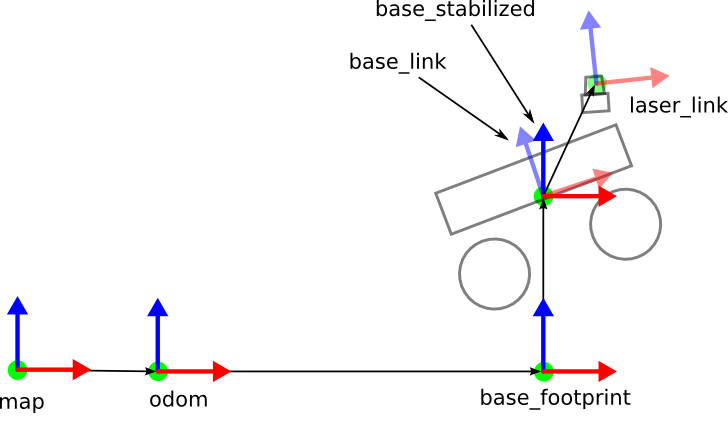
\includegraphics[width=.5\linewidth]{images/tf.png}
	\caption{transform of robot points.\cite{tfrobot}}
\end{figure}

Hector mapping needs laser input published over the laser scan node, and also \textit{tf} (transform) information about the robot. The \textit{tf} represents the difference in height of the laser from the ground or an offset in $x$, $y$ and $z$ coordinates. A robotic arm with multiple joints would have a transform on each of them so the system could calculate movement of the sensor located on the arm.

\begin{figure}[H]
	\centering
	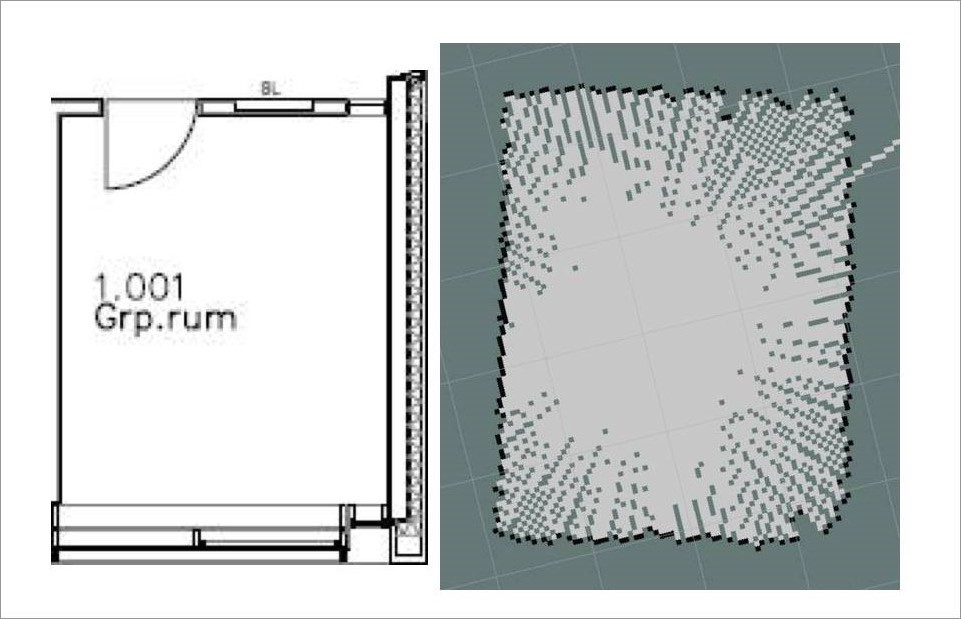
\includegraphics[width=.5\linewidth]{images/compare.jpg}
	\caption{Room-plan of H101, Aalborg University Esbjerg.}
\end{figure}

We took a single measurement using the laser and hector SLAM, which created the map shown to the left on the figure above. The university gave us a picture of group room H101 at Aalborg University Esbjerg, which we used to compared the map from Hector SLAM with the floor plan. 

\begin{figure}[H]
	\centering
	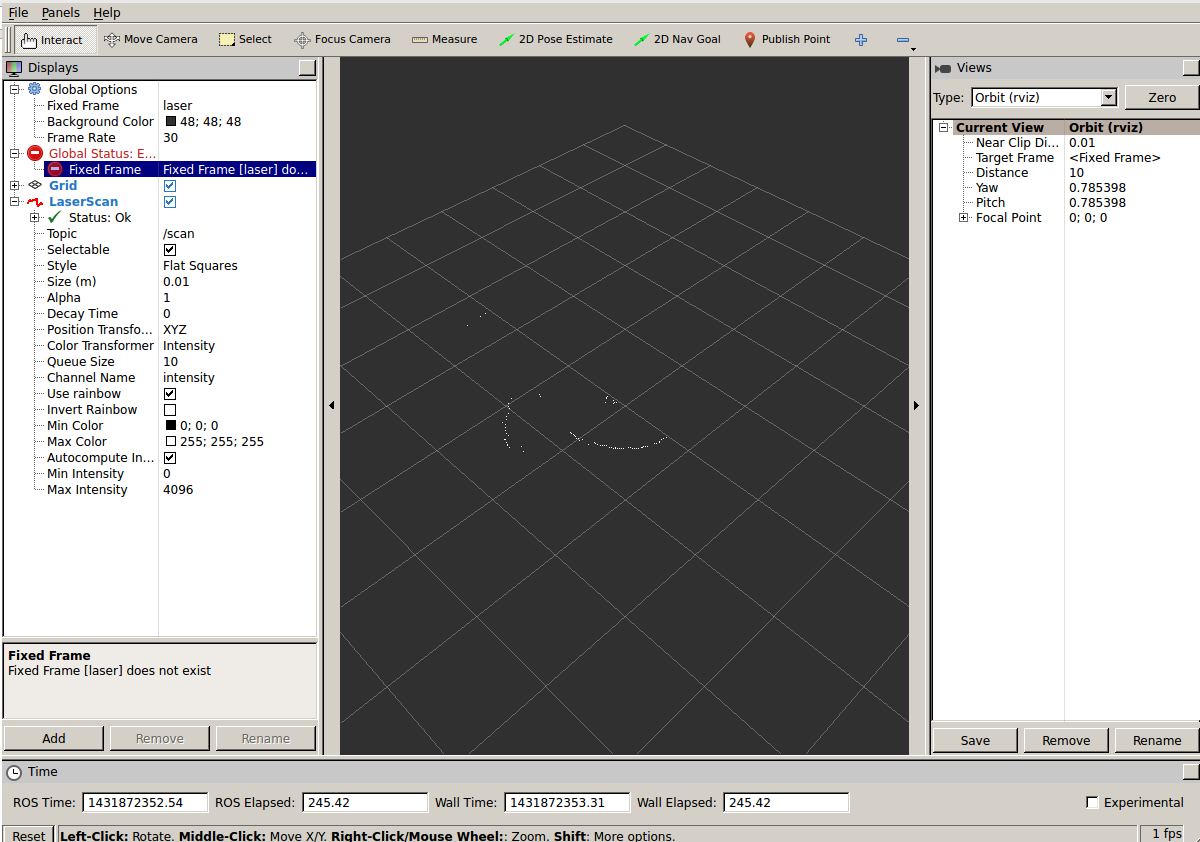
\includegraphics[width=.5\linewidth]{images/rviz.png}
	\caption{Rviz visualization tools package in ROS.}
\end{figure}

The Hector map picture is a screen shot taken from rviz. Rviz is a visualization tool included in ROS, which allows the user to see the laser measurements and 2D mapping in real-time.\cite{rviz}

Hector mapping takes the information given from the transform and laser measurement and makes a 2D map from it. The following figure is a flow-chart explaining these steps.

\begin{figure}[H]
	\centering
	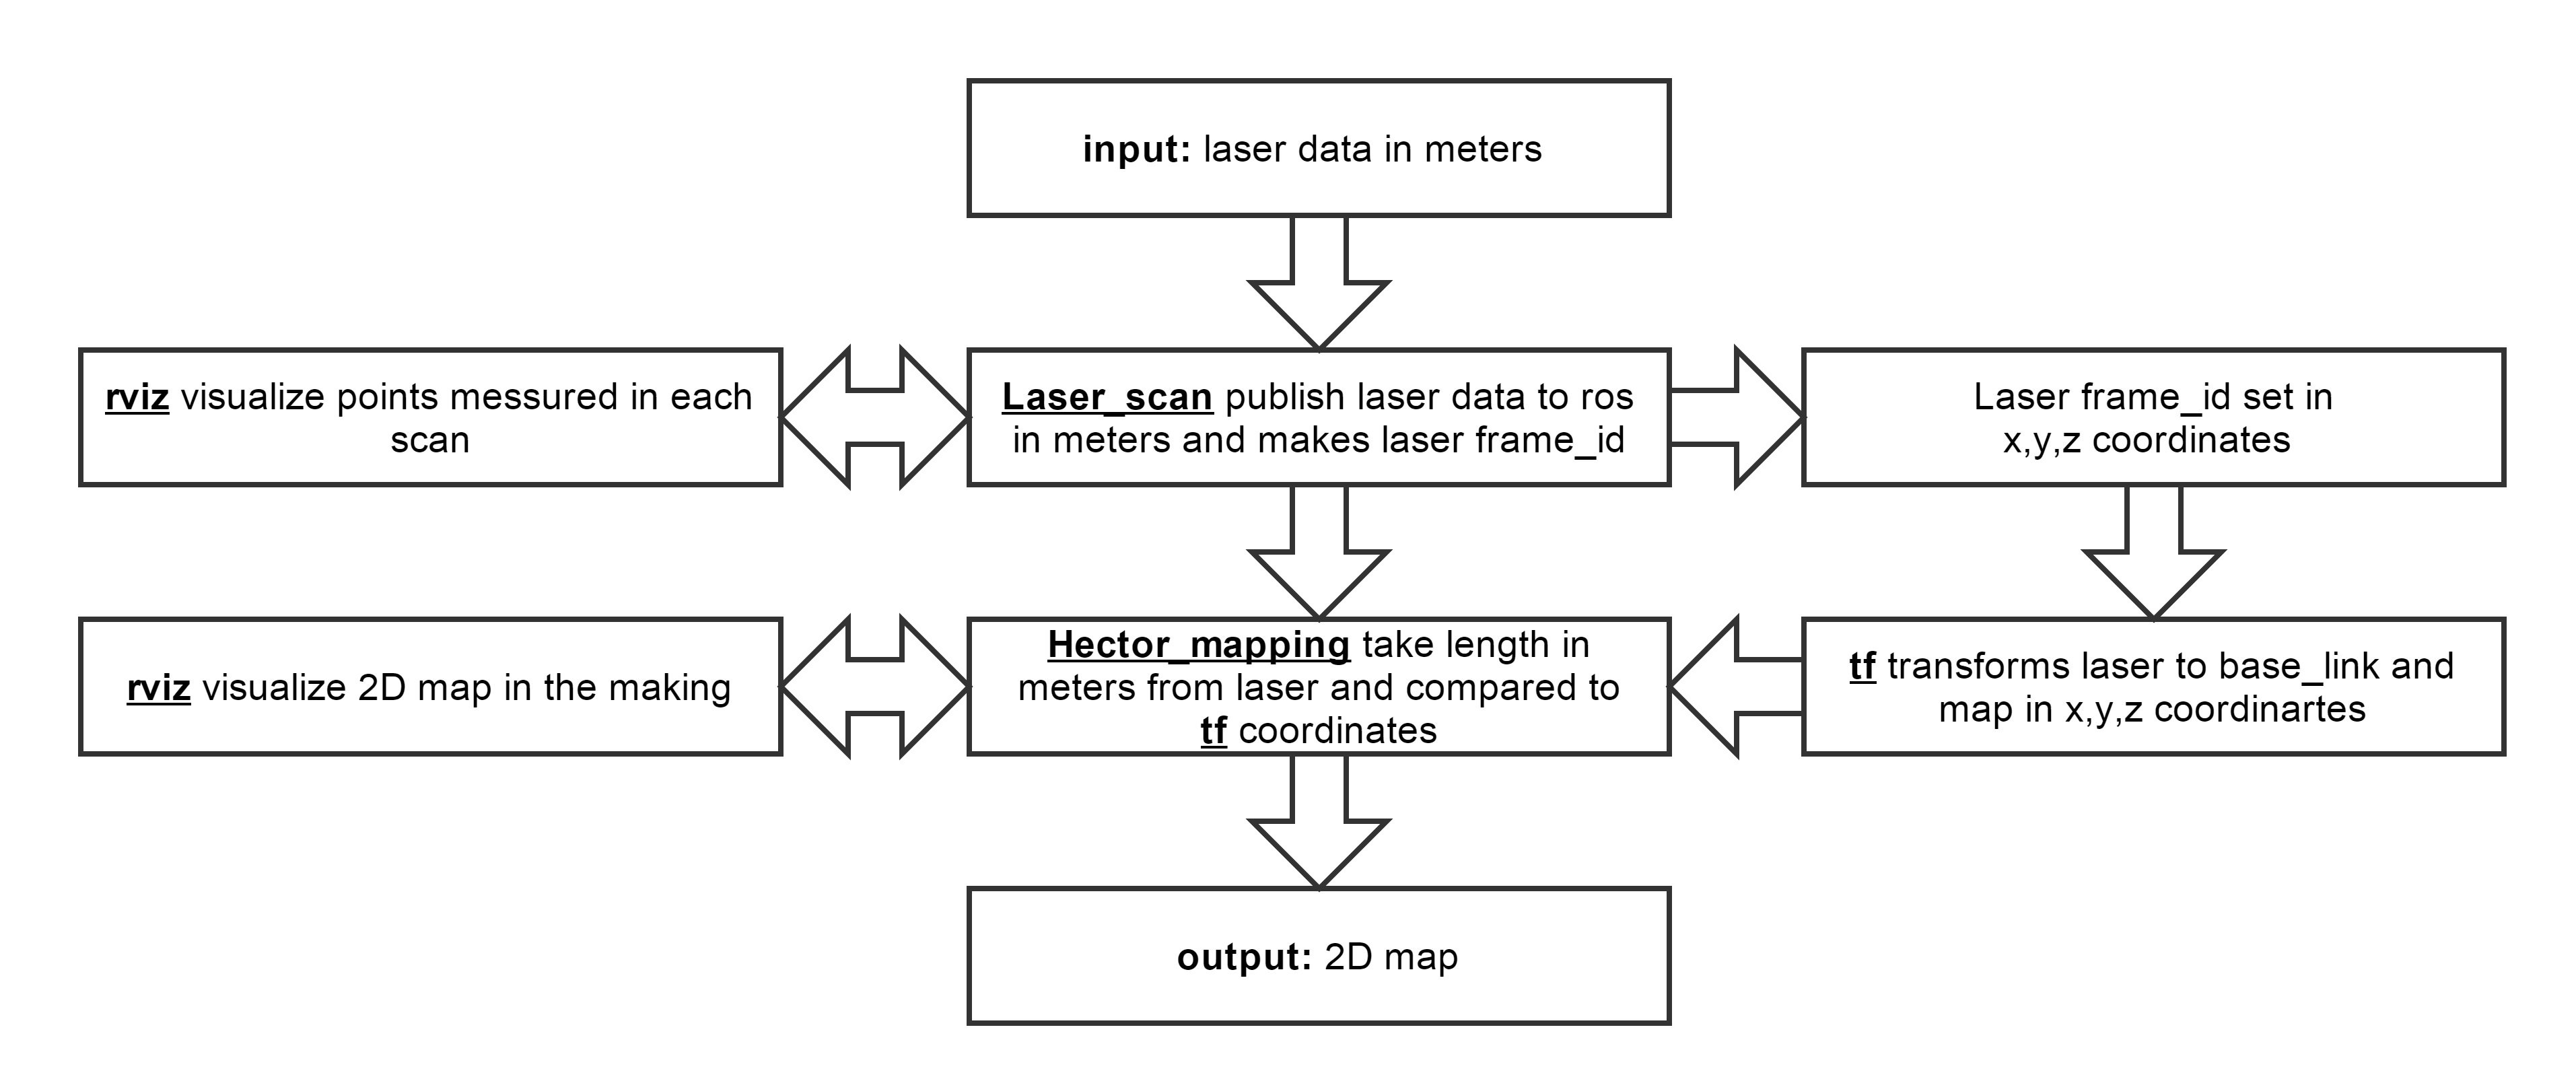
\includegraphics[width=1\linewidth]{images/hector_flow.png}
	\caption{Hector mapping flowchart.}
\end{figure}

We made a .bag file recording the $/$scan topic on the raspberry pi, then it was copied to a laptop running ubuntu and ros. The bag file was played on the laptop and hector mapping, with transform published, was run. The outcome was a hector map. 

\lstinputlisting[firstline=1, lastline=19, title=main.launch, language=xml]{../code/main.launch} 
